\chapter{Diversidad de Rango}

Los primeros análisis se enfocaron en buscar hechos relevantes que propiciaron las migraciones de palabras,  siendo oportuna la información histórica.  El capítulo anterior busco ver a cada idioma como un conjunto “universal” donde las propiedades que lo caracterizan  son comunes en cada uno y siguen siendo válidas a pesar de reducir los elementos que los componen al extraer palabras. 

En esta sección se buscará entender cómo son las variaciones de palabras a  lo largo del tiempo, para ello  se enfocara el estudio a cuantificar que tan diferentes son las listas de los préstamos de un idioma en otro,  ya que estas listas están ordenadas por rango, (donde el rango más bajo es la palabra más común en ese año y la de rango más alto la menos utilizada)  una misma palabra puede ocupar distintos cargos en diferentes años,  o  para un mismo rango existe una diversidad de palabras que lo ocupan, esta idea es más adecuada ya hay palabras que no  aparecen en todos los años del análisis,  sin embargo en todos las listas  hay palabras hasta cierta posición (rango).   

La propuesta de la diversidad de rango ha utilizada en idiomas y en deportes [XXXX], siendo útil para mostrar características comunes de los conjuntos donde es medida.  El algoritmo para llegar a la diversidad se propuso en [XXX], y se describe de la siguiente manera:


\begin{enumerate}
	
	\item Se fijan un año inicial $t_{o}$ y uno final $t_{o}$, construyendo un intervalo de años a evaluar $\Delta\,t = t_{f}- t_{o}$.
	
	\item Se toma el primer rango de todos los años en el intervalo y se cuenta el número de palabras que son distintas en ese rango. Esta cantidad será la diversidad para el rango uno.
	
	\item Se prosigue con el segundo rango y se vuelve a contar cuántas palabras son diferentes en todo el periodo de tiempo.  Con ello se obtiene la diversidad para el rango dos. 
	
	\item Ya que las listas de préstamos de un idioma en otro no son homogéneas en cantidad, el procedimiento anterior se repetirá hasta el rango mínimo que poseen todas las listas,  así se asegura tener una homogeneidad en el tamaño.
	
	\item Se normalizan  los valores dividiendo cada resultado entre el número de años comprendidos del intervalo $\Delta\,t$, obteniendo  la diversidad de rango $d(k)$.
	
	
\end{enumerate}


Antes de mostrar los resultados, se espera  que los valores de $d(k)$ sean cercanos a cero cuando  para un rango $k$, las cantidad de palabras que ocupan ese rango sea menor. En caso de que la diversidad sea cercana a uno,  significa que hay una mayor cantidad de palabras que ocupan el rango $k$. 


Tras graficar el rango contra la diversidad, se observó que en todas las combinaciones (a pesar de que algunas tuvieran más datos)  la tendencia de la diversidad  se asemeja a una función de distribución cumulativa logarítmica  normal, la cual depende del rango $k$, y la desviación estándar $\sigma$.

\begin{equation}
	\label{ec.cumulativa}
	F(k) = \Phi \left ( \frac{ln(k)}{\sigma} \right )\,\,\,\,k\geq 0; \sigma \geq 0
\end{equation}

Donde $\Phi$ es la función cumulativa de la distribución normal, que ademas del rango y la desviación estándar, depende del promedio $\mu$.

\begin{equation}
	\label{ec.distribucionnormal}
	\Phi(t) = \frac{1}{\sigma\sqrt{2\pi}} \int_{-\infty}^{t}  e^{ \frac{ - \left ( x-\mu \right )^{2}}{2\sigma^2}  } dx	
\end{equation}


\newpage
\subsubsection*{Ajuste de Datos }


Se intentó ajustar los puntos de la diversidad con esta distribución, sin embargo al ser pocos los rangos (la mayor cantidad de rangos en cualquier combinación fue de 250),  la curva descrita  no ajusta correctamente;  si se tuvieran mayor cantidad de rangos (1000 o 1000) del orden de $10^{3}$ o $10^{4}$ el ajuste es más preciso.  Para solucionar este problema se propuso hacer un ajuste lineal con la función logarítmica  de la siguiente forma:


\begin{enumerate}
	\item Se propone una función para la diversidad $d(k)$ de la forma
	
	\begin{equation}
	\label{ec.ajuste}
	y(k) =  \alpha \, ln(k) + \beta
	\end{equation}
	
	\item Al realizar los cambios de variable $\hat{Y} = y(k)$ y $X = ln(k)$, se obtiene una ecuación lineal para $k$.
	$$ \hat{Y} =  \alpha X + \beta$$
	
	\item Para encontrar los parámetros $\alpha$ y $\beta$, se utilizó el método de mínimos cuadrados, minimizando la suma de los cuadrados de los errores.  
	
	\item Conocidos los valores de $X$, la diversidad $Y$ y la cantidad de valores $n$,  se calcularon los valores muestrales de las medias ($\mu_{X}$ y $\mu_{Y}$), las varianzas ($\sigma^{2}_{X}$ $\sigma^{2}_{Y}$)  y la covarianza de las dos variables  $\sigma_{XY}$.
	
	$$ \bar{X} = \frac{1}{n} \sum_{i=1}^{n} X_{i} $$
	
	$$ \bar{Y} = \frac{1}{n} \sum_{i=1}^{n} Y_{i} $$
	
	$$ \sigma^{2}_{X} = \frac{1}{n} \sum_{i=1}^{n} \left (X_{i} -\bar{X}\right )^{2} $$
	
	$$ \sigma^{2}_{Y} = \frac{1}{n} \sum_{i=1}^{n} \left (Y_{i} -\bar{Y}\right )^{2} $$
	
	$$ \sigma_{XY} = \frac{1}{n} \sum_{i=1}^{n} \left (X_{i} - \bar{X}\right )  \left (Y_{i} - \bar{Y} \right ) $$
	
	\item Así los parámetros se expresan como
	
	$$ \alpha = \frac{\sigma_{XY}}{\sigma^{2}_{X}} $$
	
	$$ \beta = \bar{Y} - \alpha \bar{X}$$
	
	\item Calculados cada punto del ajuste (\ref{ec.ajuste}) $y_{i}$ y los valores calculados de diversidad $f_{i}$, para comprobar que tan adecuado es el ajuste se obtiene el coeficiente de determinación $R^{2}$.
	
	\begin{equation}
	\label{ec.rcuadrado}
	R^{2} = \frac{\sigma_{XY}}{\sigma^{2}_{X} \sigma^{2}_{Y}} \,\, = \,\, 1- \frac{\sum_{i=1}^{n} \left( y_{i} - f_{i}\right)^{2} }{\sum_{i=1}^{n} \left (y_{i} -\bar{Y}\right )^{2}}
	\end{equation}
	
	
	 
\end{enumerate}


Valores de $R^{2}$ próximos a 1 indicarán que existe una relación lineal ( en este caso logarítmica por el cambio de variable) exacta entre las dos variables

Las posteriores gráficas corresponden a las diferentes combinaciones entre idiomas orígenes y los receptores donde se calculó la diversidad de rango y el ajuste correspondiente.  Por cada conjunto de gráficas se muestra una tabla con los diferentes parámetros, la media $\mu$, la desviación estándar $\sigma$, el rango minimo donde se buscó la diversidad $k_{min}$, los parámetros del ajuste $\alpha$ y $\beta$  y el coeficiente de determinación $R^{2}$.
 
\newpage

\begin{figure}[h!]
	\centering
	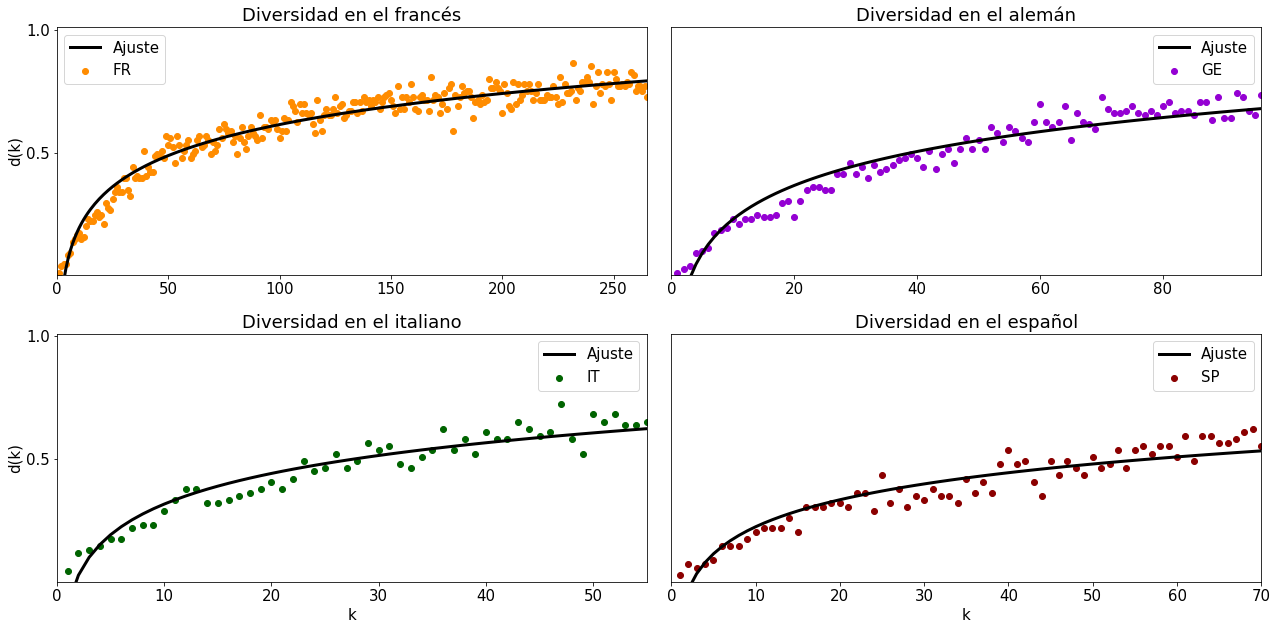
\includegraphics[width=15cm, height=6.8cm]{Cap_6/DR_EN.png}
	\label{fig.DR_EN}
	\caption{Diversidad de rango del inglés en los demás idiomas.}
\end{figure}


\begin{table}[h!]
	\centering
	\begin{tabular}{ccccccc}
		\textbf{}                & \textbf{$\mu$} & \textbf{$\sigma$} & \textbf{$k_{min}$} & \textbf{$\alpha$} & \textbf{$\beta$} & \textbf{$R^{2}$} \\
		\textbf{inglés-francés}  & 0.61           & 0.18                & 265                   & 0.18           & -0.23         & 0.94        \\
		\textbf{inglés-alemán}   & 0.49           & 0.19                & 96                    & 0.19           & -0.23         & 0.92        \\
		\textbf{ingles-italiano} & 0.45           & 0.17                & 55                    & 0.17           & -0.10         & 0.91        \\
		\textbf{ingles-español}  & 0.38           & 0.15                & 70                    & 0.15           & -0.14         & 0.88       
	\end{tabular}
	\caption{Parámetros de la diversidad del inglés en los demás idiomas.}
	\label{tab.DR_EN}
\end{table}



\newpage

\begin{figure}[h!]
	\centering
	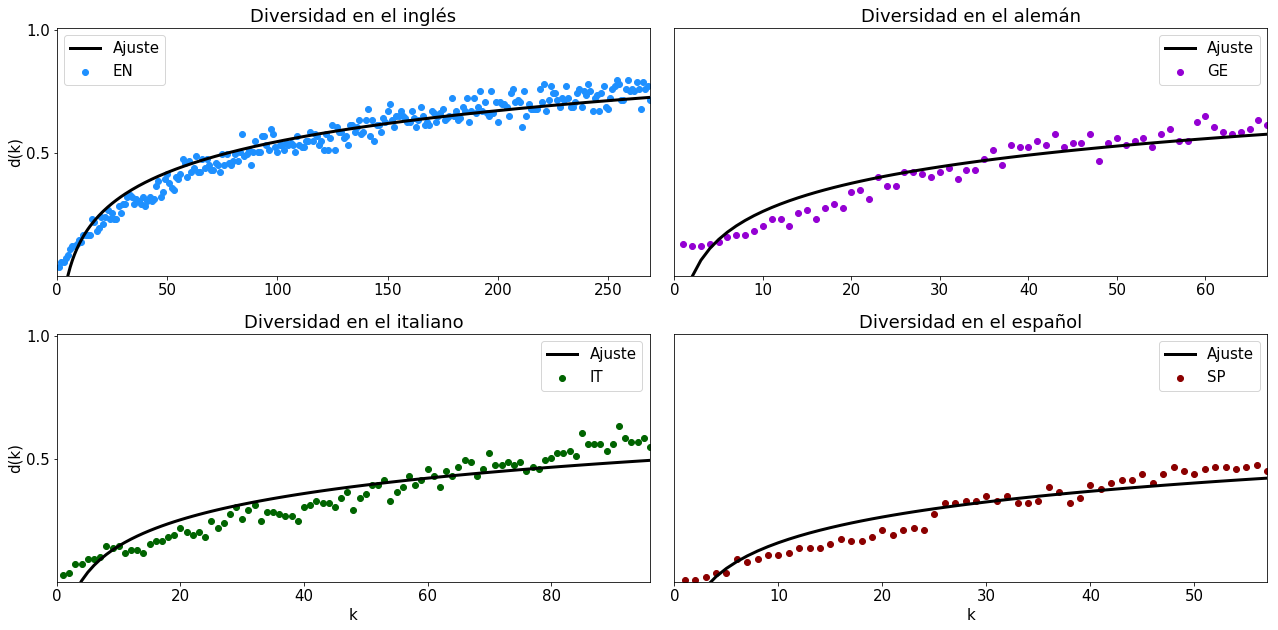
\includegraphics[width=1 \textwidth, scale = .38]{Cap_6/DR_FR.png}
	\label{fig.DR_FR}
	\caption{Diversidad de rango del francés en los demás idiomas.}
\end{figure}


\begin{table}[h!]
	\centering
	\begin{tabular}{ccccccc}
		\textbf{}                & \textbf{$\mu$} & \textbf{$\sigma$} & \textbf{$k_{min}$} & \textbf{$\alpha$} & \textbf{$\beta$} & \textbf{$R^{2}$} \\
		\textbf{francés-inglés}  & 0.55           & 0.18                & 269                   & 0.18           & -0.29        & 0.93        \\
		\textbf{francés-alemán}   & 0.42           & 0.16                & 67                    & 0.17           & -0.12         & 0.87        \\
		\textbf{francés-italiano} & 0.35           & 0.16                & 96                    & 0.15           & -0.21         & 0.83        \\
		\textbf{francés-español}  & 0.28           & 0.14                & 57                    & 0.15           & -0.19         & 0.86       
	\end{tabular}
	\caption{Parámetros de la diversidad del francés en los demás idiomas.}
	\label{tab.DR_FR}
\end{table}


\newpage

\begin{figure}[h!]
	\centering
	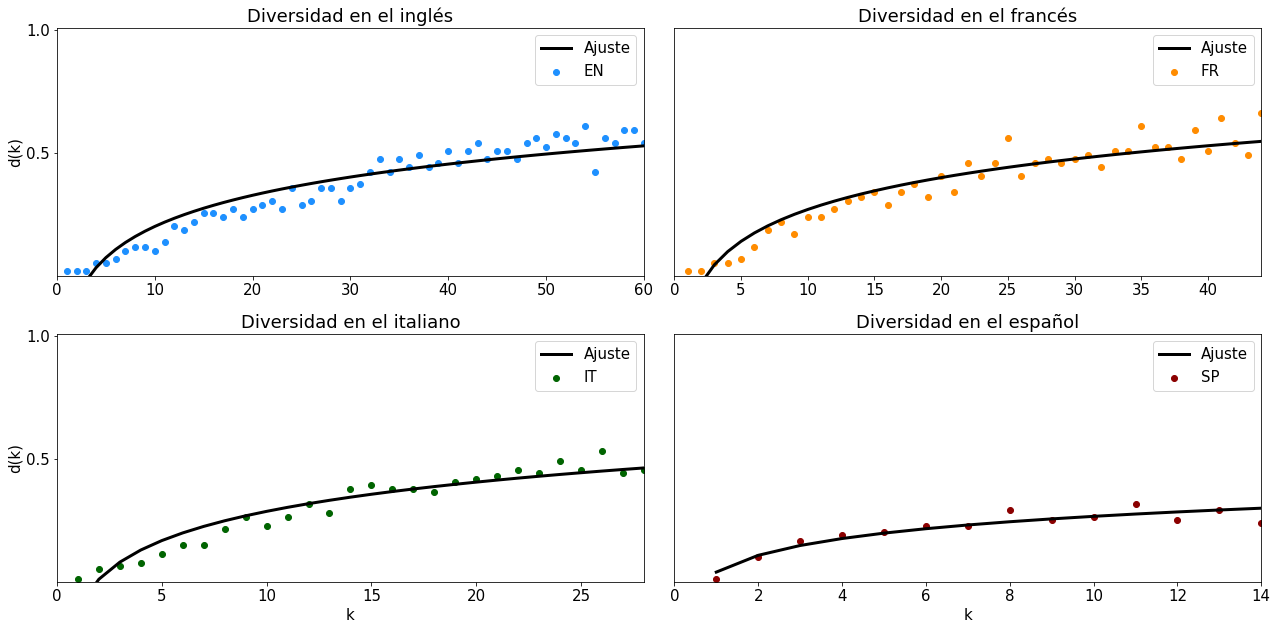
\includegraphics[width=1 \textwidth, scale = .38]{Cap_6/DR_GE.png}
	\label{fig.DR_GE}
	\caption{Diversidad de rango del alemán en los demás idiomas.}
\end{figure}


\begin{table}[h!]
	\centering
	\begin{tabular}{ccccccc}
		\textbf{}                & \textbf{$\mu$} & \textbf{$\sigma$} & \textbf{$k_{min}$} & \textbf{$\alpha$} & \textbf{$\beta$} & \textbf{$R^{2}$} \\
		\textbf{alemán-inglés}  & 0.35          & 0.17                & 60                   & 0.18           & -0.22        & 0.88        \\
		\textbf{alemán-francés}   & 0.37           & 0.17                & 44                    & 0.19           & -0.16         & 0.89        \\
		\textbf{alemán-italiano} & 0.31           & 0.15                & 28                    & 0.17           & -0.11         & 0.91        \\
		\textbf{alemán-español}  & 0.22          & 0.08                & 14                    & 0.10           & -0.04         & 0.89       
	\end{tabular}
	\caption{Parámetros de la diversidad del alemán en los demás idiomas.}
	\label{tab.DR_GE}
\end{table}


\newpage

\begin{figure}[h!]
	\centering
	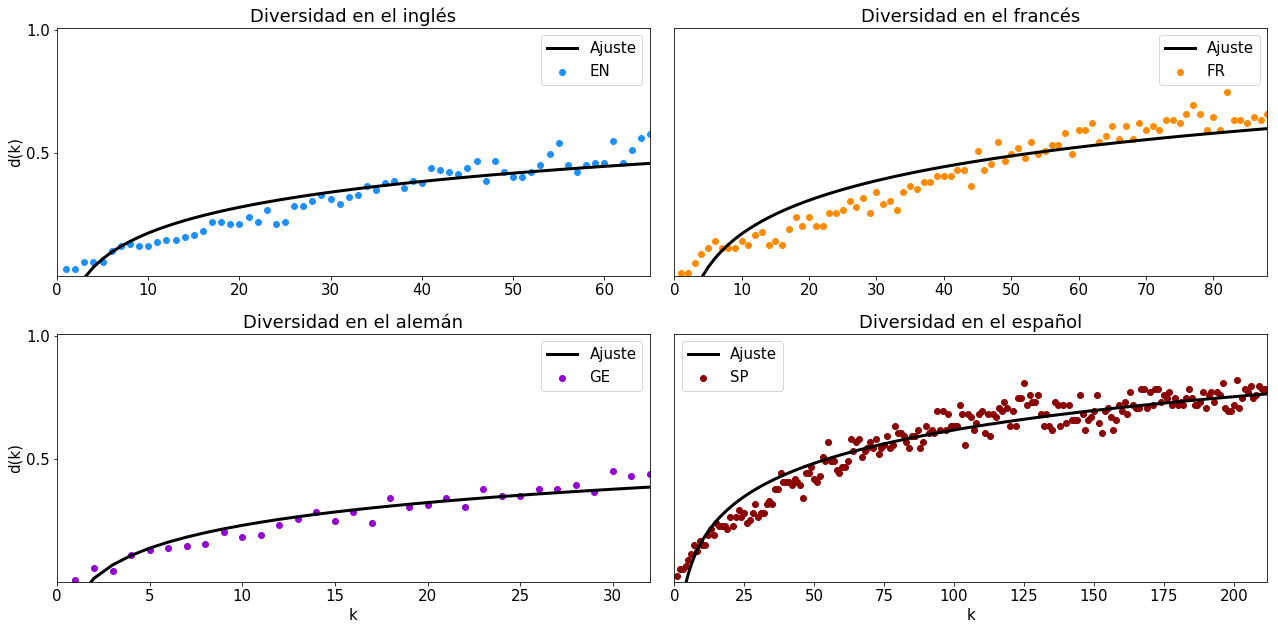
\includegraphics[width=1 \textwidth, scale = .38]{Cap_6/DR_IT.png}
	\label{fig.DR_IT}
	\caption{Diversidad de rango del italiano en los demás idiomas.}
\end{figure}


\begin{table}[h!]
	\centering
	\begin{tabular}{ccccccc}
		\textbf{}                & \textbf{$\mu$} & \textbf{$\sigma$} & \textbf{$k_{min}$} & \textbf{$\alpha$} & \textbf{$\beta$} & \textbf{$R^{2}$} \\
		\textbf{italiano-inglés}  & 0.31          & 0.15                & 66                   & 0.15           & -0.18        & 0.86        \\
		\textbf{italiano-francés}   & 0.41           & 0.20                & 88                    & 0.20           & -0.28         & 0.85        \\
		\textbf{italiano-alemán} & 0.26           & 0.12                & 32                    & 0.13           & -0.08         & 0.91        \\
		\textbf{italiano-español}  & 0.22          & 0.19                & 212                    & 0.20           & -0.28         & 0.92       
	\end{tabular}
	\caption{Parámetros de la diversidad del italiano en los demás idiomas.}
	\label{tab.DR_IT}
\end{table}


\newpage

\begin{figure}[h!]
	\centering
	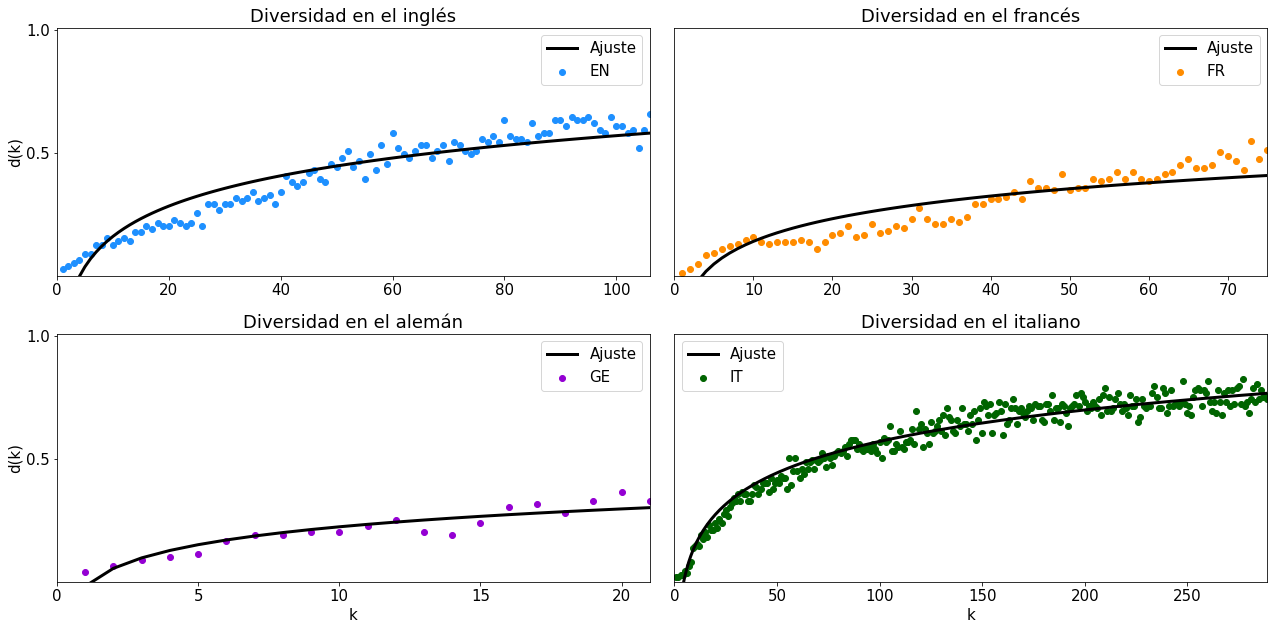
\includegraphics[width=1 \textwidth, scale = .38]{Cap_6/DR_SP.png}
	\label{fig.DR_SP}
	\caption{Diversidad de rango del español en los demás idiomas.}
\end{figure}


\begin{table}[h!]
	\centering
	\begin{tabular}{ccccccc}
		\textbf{}                & \textbf{$\mu$} & \textbf{$\sigma$} & \textbf{$k_{min}$} & \textbf{$\alpha$} & \textbf{$\beta$} & \textbf{$R^{2}$} \\
		\textbf{español-inglés}  & 0.41          & 0.18                & 106                   & 0.18           & -0.25        & 0.87        \\
		\textbf{español-francés}   & 0.28           & 0.14                & 75                   & 0.13           & -0.17         & 0.79        \\
		\textbf{español-alemán} & 0.21           & 0.09                & 21                    & 0.11           & -0.02         & 0.86        \\
		\textbf{español-italiano}  & 0.22          & 0.18                & 289                    & 0.18           & -0.28         & 0.95       
	\end{tabular}
	\caption{Parámetros de la diversidad del español en los demás idiomas.}
	\label{tab.DR_SP}
\end{table}